\section{Data Analysis}

Now we aim to dissect our dataset to reveal how users use their wishlists. Particularly we are interested in the products user prefer to buy, as well as the time that is appealing to shoppers. We compare user preferences in 3 different regions to show market trend. Besides, we also quantify the increase in different time of a year. Specifically we show different shopping behaviors in various holidays.

\subsection{Basic Statistics}
First we conduct fundamental measurements on the dataset to help build basic understanding on how wishlists are used and to what extend the users expose their personal information in Amazon. 

For all 967,603 users collected in the first step of data collection, we record totally 2,121,173 wishlists and 5,700,000 items (in which 2,248,142 items are unique). We show distribution metrics in Table~\ref{tb:stat2}. As we can see from the table, every user has 2.56 wishlists in average with standard deviation of 4.97. The average number and standard deviation of items in a wishlist is 74.2 and 187.3 accordingly. And the average and standard deviation of product price is \$35.06 and 172.0. Note that although we list the maximum number of wishlists a user has (Similarly, items in wishlists and item price) in our dataset, we did not probe the limit set by Amazon. All three distributions have very high skewness~($\gamma_1$) and kurtosis~($\kappa$), which means the distributions are very skewed and heavily tailed. For clearer presentation, we show the distribution of wishlist in Figure~\ref{avglist}, distribution of items in Figure~\ref{avgitem}, and distribution of price in Figure~\ref{avgprice} using log-scaled y axis.

\begin{table}[!htbp]
\centering
\caption{Distributions}
\label{tb:stat2}
\begin{adjustbox}{max width=.5\textwidth}
\begin{tabular}{llllll}
Distribution & Mean & Max & SD & $\gamma_1$ & $\kappa$ \\ \hline
Wishlist in Profile & 2.56 & 326 & 4.97 & 19.7 & 854.15 \\
Items in Wishlist & 74.2 & 7,350 & 187.3 & 8.25 & 111.11 \\
Item Price & 35.06 & 105,065 & 172.0 & 299.4 & 144,743.2 \\
\end{tabular}
\end{adjustbox}
\end{table}

\begin{figure*}[!htb]
\minipage{0.32\textwidth}
  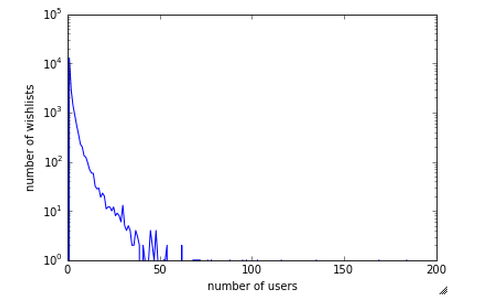
\includegraphics[width=\linewidth]{avglist.png}
  \caption{Number of lists the users have}\label{avglist}
\endminipage\hfill
\minipage{0.32\textwidth}
  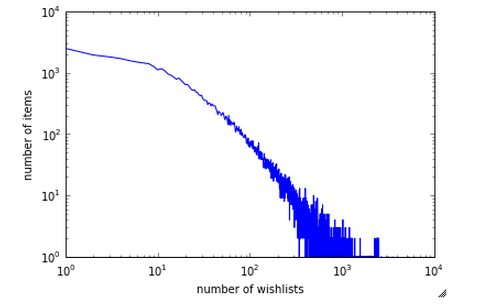
\includegraphics[width=\linewidth]{avgitem.png}
  \caption{Number of items the lists have}\label{avgitem}
\endminipage\hfill
\minipage{0.32\textwidth}%
  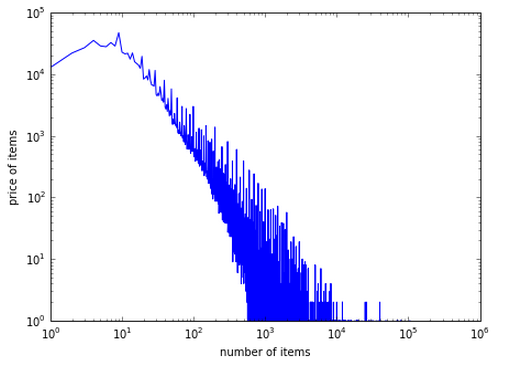
\includegraphics[width=\linewidth]{avgprice.png}
  \caption{Item Price}\label{avgprice}
\endminipage
\end{figure*}


\subsection{User preference}
A core question on user preference is what the users would like to buy and how much they are willing to pay for certain products. To categorize the products, we directly use item type that are in the product pages (See Fig~\ref{item}. From all product pages that are visited we found 50 types in total. Note that Amazon was reported to do price discrimination on E-books~\cite{mikians2012detecting}, which indicates a same E-book may be priced differently in various locations. However, these locations are in scope of countries. In our study, we focus on the U.S. Besides, we believe our results are also meaningful in a global perspective since only E-books are price discriminated. Most of our conclusions still stand.

We show national user preference in Table~\ref{tb:overall}. With over 40\% of items in wishlist being books, we can see books are in domination. Beside normal paperback books, E-books in Kindle are also being very popular. We believe the cheap price of E-book is a main reason for its prosperity (Books are 136.7\% more expensive than E-books in average). Other than books, entertainment products play second important roles. Movies \& TV, CDs \& Vinyl, Toys \& Games, and Video games rank 2, 4, 5, 6 accordingly, which indicate that users are normally pursuing leisure products on Amazon. The following popular products are fashions, home related, and sport items. We also found that Computers, All Electronics, and Camera are only 3 types of products users are paying more than \$100 in average, which shows that users are paying substantially more in electronic devices than other products.


\begin{table}[!ht]
\centering
\caption{Overall User Preference}
\label{tb:overall}
\begin{adjustbox}{max width=.5\textwidth}
\begin{tabular}{lllll}
Rank & Item Type          & Number of Items & Percentage of Items & Average Price(\$) \\ \hline
1 & Books & 1829657 & 41.55\% & \$22.25 \\
2 & Movies \& TV & 533504 & 12.12\% & \$25.26 \\
3 & Buy a Kindle & 391967 & 8.90\% & \$9.40 \\
4 & CDs \& Vinyl & 337188 & 7.66\% & \$17.36 \\
5 & Toys \& Games & 231522 & 5.26\% & \$40.42 \\
6 & Video Games & 103951 & 2.36\% & \$46.87 \\
7 & Amazon Fashion & 102012 & 2.32\% & \$57.77 \\
8 & Kitchen \& Dining & 99647 & 2.26\% & \$46.00 \\
9 & Sports \& Outdoors & 95522 & 2.17\% & \$59.16 \\
10 & Home \& Kitchen & 85088 & 1.93\% & \$58.50 \\
11 & Home Improvement & 72194 & 1.64\% & \$62.49 \\
12 & All Electronics & 58146 & 1.32\% & \$121.55 \\
13 & Health \& Personal Care & 47912 & 1.09\% & \$34.54 \\
14 & Digital Music & 38375 & 0.87\% & \$8.94 \\
15 & Computers & 38066 & 0.86\% & \$123.31 \\
16 & All Beauty & 37946 & 0.86\% & \$23.45 \\
17 & Camera \& Photo & 37725 & 0.86\% & \$192.99 \\
18 & Arts, Crafts \& Sewing & 31029 & 0.70\% & \$24.91 \\
19 & Patio, Lawn \& Garden & 30747 & 0.70\% & \$66.83 \\
20 & Grocery \& Gourmet Food & 27616 & 0.63\% & \$21.67 \\
\end{tabular}
\end{adjustbox}
\end{table}

After analyzing the general shopping preference of Amazon users, it is natural to study the preferences of people from different demographical and geographical groups. For demographical factor, we compare the shopping preference of males and females. For geographical factor, we compare customers from 3 different geo-location, which are -- east coast \cite{east}, west coast\cite{west}, and middle of the US. 

\subsubsection{Different Gender}
To start with, we show the top 10 popular products of male users in Table~\ref{tb:male} and female users in Table~\ref{tb:female}. In addition, the average product price for male and female is \$36.95 and \$26.53 correspondingly. Clearly we can find that male and female customers have different shopping preference. First of all, products in males' wishlists have 39.3\% higher price than those in females' wishlists averagely. Furthermore, males are willing to pay higher price in all categories in the two tables. The gap between the product price is even larger than the income gap between males and females, which are reported that males earn 21.1\% more than females in 2014~\cite{menvswomen}. Therefore we concluded that males are prone to spend more online. Beside the price difference, different genders also prefer different categories of products. While ``Books" and ``Buy a Kindle" account around 50\% of the products for both genders, male customers are more likely to buy a paperback book instead of E-books than female customers. Males prefer sports and electronics while females prefer fashions and beauty-related items. Interestingly, females like ``Arts, Crafts \& Sewing" much more than males as such items count only 0.3\% of all products and ranks 26 in all categories for males. In general, 13 out of the most popular 24 categories (both male and female have over 5000 products in these categories) have over 100\% difference, which means that the percentage of certain product of a gender is at least double as the other gender. 

\begin{table}[!ht]
\centering
\caption{Male User Preference}
\label{tb:male}
\begin{adjustbox}{max width=.5\textwidth}
\begin{tabular}{lllll}
Rank & Item Type          & Number of Items & Percentage of Items & Average Price(\$) \\ \hline
1 & Books & 1306784 & 43.56\% & \$24.16 \\
2 & Movies \& TV & 386769 & 12.89\% & \$26.01 \\
3 & CDs \& Vinyl & 264310 & 8.81\% & \$18.10 \\
4 & Buy a Kindle & 208003 & 6.93\% & \$10.60 \\
5 & Toys \& Games & 142277 & 4.74\% & \$44.52 \\
6 & Video Games & 81003 & 2.70\% & \$48.13 \\
7 & Sports \& Outdoors & 76039 & 2.53\% & \$61.28 \\
8 & Home Improvement & 59606 & 1.99\% & \$65.00 \\
9 & All Electronics & 48746 & 1.62\% & \$126.75 \\
10 & Amazon Fashion & 48251 & 1.61\% & \$69.00 \\
\end{tabular}
\end{adjustbox}
\end{table}


\begin{table}[!ht]
\centering
\caption{Female User Preference}
\label{tb:female}
\begin{adjustbox}{max width=.5\textwidth}
\begin{tabular}{lllll}
Rank & Item Type          & Number of Items & Percentage of Items & Average Price(\$) \\ \hline
1 & Books & 493964 & 37.22\% & \$17.50 \\
2 & Buy a Kindle & 176831 & 13.32\% & \$8.00 \\
3 & Movies \& TV & 137732 & 10.38\% & \$23.30 \\
4 & Toys \& Games & 82399 & 6.21\% & \$33.71 \\
5 & CDs \& Vinyl & 68012 & 5.12\% & \$14.65 \\
6 & Amazon Fashion & 51788 & 3.90\% & \$48.08 \\
7 & Kitchen \& Dining & 49058 & 3.70\% & \$38.30 \\
8 & Home \& Kitchen & 42372 & 3.19\% & \$50.04 \\
9 & All Beauty & 25440 & 1.92\% & \$21.74 \\
10 & Arts, Crafts \& Sewing & 21475 & 1.62\% & \$22.51 \\
\end{tabular}
\end{adjustbox}
\end{table}

\subsubsection{Different Region}

After presenting strong variances in gender preference with quantitative analysis. We now show geographical difference among 3 regions as mentioned -- east coast, west coast, and the US. Note that only \%57 users have location information in their list descriptions. Following analysis include only the users that input their locations. Due to space limitation we do not show all popular products. Instead we present some of the interesting observations. 

The total amount of items from east coast, west coast, and mid of US are 641,252, 420,828, and 1,109,846. The average product price in east coast, west coast, and mid of US are \$35.80, \$35.83, and \$33.45. While users from east coast and west coast have almost the same product price, users in the middle of US expose highest price sensitivity -- they prefer to pay 6.6\% less than other 2 groups in products they desire. It also agrees with the common knowledge that coastal areas have higher income than mid area. However, generally the distributions of items are very similar in the 3 regions. Some noteworthy differences are (1) users from east coast has 2.66\% ``sports \& Outdoors" products. The percentage is 14.2\% and 33.0\% more than that of west coast and mid of the U.S. However, they are prone to pay 8.4\% and 7.9\% less in these products. (2) West coastal users are willing to pay \$70.88 in ``Home Improvement" products, which are 12.9\% and 22.8\% more than east and mid area. The percentage of ``Home Improvement" is also higher (1.92\% compared to 1.49\% in mid area and 1.72\% in east coast). 

To conclude, we show that different genders expose vastly different online shopping preference. We also show that people from 3 different regions have similar shopping pattern. Although in most cases it is true, we still point out noticeable diversity among users in these 3 regions. 

\subsection{Time Factor}
After analyzing product categories and price, we study another important factor that describes user behaviors -- time factor. We explore shopping trend during weekdays and weekends, as well as normal days and holidays. By investigating the added date of items we learn the days that are most appealing to shoppers. 

\subsubsection{Weekdays and Weekends}



\begin{figure}[h!]
\centering
  \caption{Items Added in Weekdays and Weekends}{}
  \label{fig:week}
  \centering
    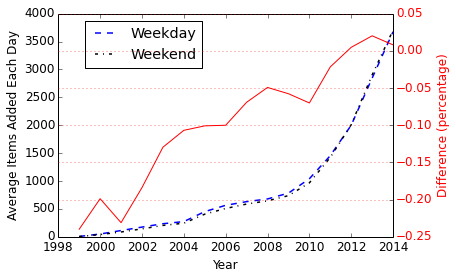
\includegraphics[width=0.45\textwidth]{weekday.png}
\end{figure}

\subsubsection{Normal days and Holidays}

In this section we measure how the items are added in the wish lists during holidays and normal days. As there are many unofficial or regional holidays, our study considers only nation-wide federal holidays. There are totally 10 qualified holidays. These holidays (http://www.usa.gov/citizens/holidays.shtml) and the date of the holidays are listed in Table~\ref{tb:holiday}.

\begin{table}[!ht]
\centering
\caption{U.S Federal Holidays}
\label{tb:holiday}
\begin{adjustbox}{max width=.45\textwidth}
\begin{tabular}{ll}
New Year's Day & January 1  \\
Birthday of Martin Luther King, Jr. & third Monday in January  \\
Washington's Birthday & third Monday of February  \\
Memorial Day & last Monday of May \\
Independence Day & July 4  \\
Labor Day & first Monday of September  \\
Columbus Day & second Monday in October  \\
Veterans Day & November 11  \\
Thanksgiving Day & fourth Thursday in November  \\
Christmas Day & December 25  \\
\end{tabular}
\end{adjustbox}
\end{table}

We analyze the data in 2 dimensions. First, We measure the items added in these holidays and compare the average items added in holidays and normal days. Then we compare the added items among different holidays. When calculating items added in a certain holiday, we consider the nearest consecutive 5 days. That is to say, we include the previous 2 days and the next 2 days in our holiday shopping session. For example, the Christmas day is December 25. We will include December 23, December 24, December 25, December 26, December 27 in Christmas day calculation. As a result, calculate items added during a year in a little different manner -- we include the last 2 days in previous year because the 2 days are considered New Year's day. We do not include the first 2 days in the next year because there is no holidays in the end of Decembers.


\subsubsection{Holidays and Normal Days}
According to our data, people start to add items in their wish lists since 1999. We analyze the items added in normal days and holidays in each year by calculating the average items added in the 2 groups. Figure~\ref{year} shows the items added in normal days and holidays 


\begin{enumerate}
\item The items added in wish lists increase year by year, no matter in normal days or holidays. We believe that the reason behind is that electric commercial gains its popularity.
\item There is increase in number of items added during holidays. The average increase rate is 10.89\%. However, as the data for year 1999 is not sufficient to be representative, we exclude year 1999 in our calculation and eventually we conclude that there is around 5.9\% increase in holidays. 
\item Generally people do buy more stuff during holidays. However, the increase is very limited. In 2001, the items added during holidays are even less than normal days. 
\end{enumerate}


\begin{figure}[h!]
\centering
  \caption{Items Added in Normal Days and Holidays}{}
  \label{fig:holiday}
  \centering
    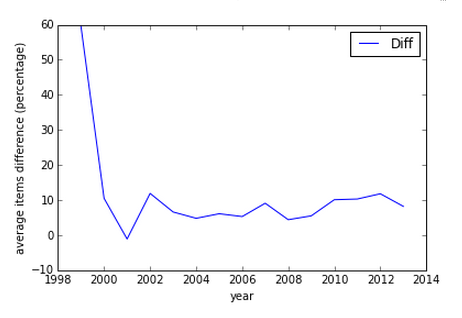
\includegraphics[width=0.45\textwidth]{holiday.png}
\end{figure}


\subsubsection{Different Holidays}
Previously we compared the shopping difference between holidays and normal days. We found that although people shop more in holidays, the increase is not that much. Our findings are against common impression that people do shop a lot in holidays, especially Thanksgiving and Christmas. We realized that it is rough to group all national holidays together to compare to normal days. We believe that holidays are also different from each other. For example people tend to shop more in Thanksgiving and Christmas. Therefore we compare different holidays in our study. Similarly, we include the last 2 days in the previous year in our analysis. There are 10 national holidays as introduced before. We again calculate the average number of items added in the nearest consecutive 5 days and compare to the average number of normal days. 

We use the data from year 1999 - 2014 and the year 2014 solely. We wish to show both the average case(from 1999-2013) and the current trend (only year 2013). We do not use data from Year 2014 because during the time of the study, the years 2014 has not been finished. Note that when computing the average item number added in normal days, we leave out all the holidays instead of simply leaving out the one that is being analyzed. The result is shown in Figure~\ref{alldiffholiday} for 1999-2013 and Figure~\ref{diffholiday} for the year 2013. In Figure~\ref{diffholiday}, The x-axis indicate the holidays accordingly (0-New Year's day, 1-Birthday of Martin Luther King, Jr, 2-Washington's Birthday, 3-Memorial Day, 4-Independence Day, 5-Labor Day, 6-Columbus day, 7-Veterans Day, 8-Thanksgiving day, 9-Christmas day).


\begin{figure}[!h]
\centering
\begin{minipage}{.25\textwidth}
  \centering
  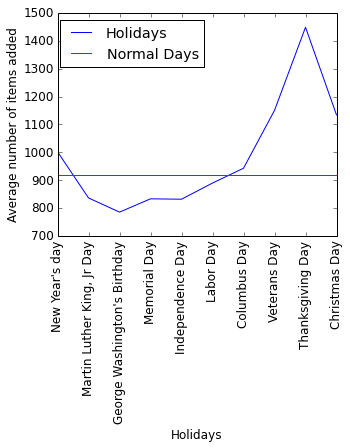
\includegraphics[width=.9\linewidth]{alldif.png}
  \captionof{figure}{Different Holidays in 1999-2014}
  \label{alldiffholiday}
\end{minipage}%
\begin{minipage}{.25\textwidth}
  \centering
  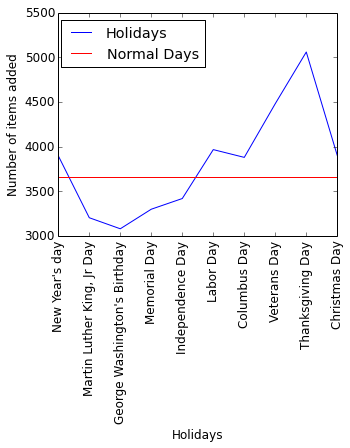
\includegraphics[width=.9\linewidth]{diff.png}
  \captionof{figure}{Different Holidays in 2014}
  \label{diffholiday}
\end{minipage}
\end{figure}


%\begin{figure}[H]
%%\minipage{0.5\textwidth}
%  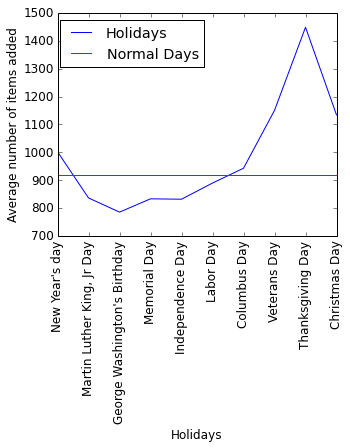
\includegraphics[width=\linewidth]{alldif.png}
%\caption{Different Holidays through 16 years}.
%\label{alldiffholiday}
%\endminipage\hfill
%\minipage{0.5\textwidth}%
%  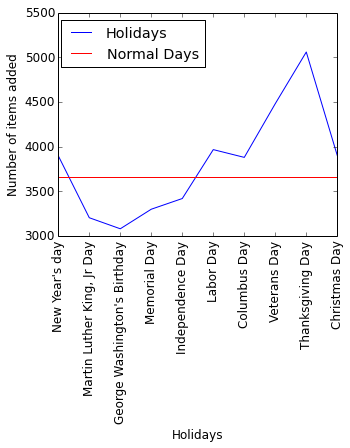
\includegraphics[width=\linewidth]{diff.png}
%\caption{Different Holidays in 2014}.
%\label{diffholiday}
%\endminipage
%\end{figure}


According to Figure~\ref{alldiffholiday} and Figure~\ref{diffholiday}, we find that holidays have huge difference between each other. In addition, we make the following observations:
\begin{enumerate}
\item The 2 figures match very well, which means that people do not tend to change their shopping behaviors at least during a short period of time. 
\item Some of the holidays are not much different from normal days (For example, Columbus Day). What is more, some of the holidays make the people less willing to add items in their wish lists. 
\item New Year's day, Veterans day, Thanksgiving, and Christmas day are 4 holidays that have quite obvious shopping increase. The result indicates that people tend to buy more stuff during the 4 holidays. The increase rate is 4.1\%, 25.2\%,72.8\%, and 30.2\% accordingly for all 15 years we analyzed. 
\item Among the 4 holidays, Thanksgiving day is the most shopping appealing holiday, which is 72.8\% higher than normal days. It is reasonable because people always get considerable discount during thanksgiving days. Christmas is the second most shopping appealing holiday because people always need to buy presents during Christmas.
\item At the first glance it is surprising that 4 holidays -- Birthday of Martin Luther King. Jr, Washington's Birthday, Memorial Day, Independence Day, and Labor day -- clearly have even less items added to user Wish Lists. The drop percentage is 10.7\%, 11.8\%, 9.0\%, 11.3\%, and 4.6\%. One possible reason is that People are more likely to be involved in other activities other than shopping during these holidays. 3 out of the 4 holidays are memorial days. Certainly these days are considered not good for shopping. 
\end{enumerate}

We believe our quantitative results are helpful in guiding merchant marketing strategies and targeted advertising. 
